\documentclass[12pt]{article}
\usepackage{graphics}
\usepackage{graphicx}
\usepackage{amsmath, amssymb}
\usepackage[margin=1.1in,footskip=.25in]{geometry}

\begin{document}
\title{Addressing Modes}
\maketitle

\section{Implied Mode}
In this mode, the operands are specified implicitly in the definition of the instruction.

\section{Immediate Mode}
In this mode, the operand is specified in the instruction itself.

$$
AC \leftarrow \#NBR
$$

\section{Register Mode}
In this mode, the operand are in registers that reside within the CPU.

$$
AC \leftarrow R1
$$

\section{Register Indirect Mode}
In this mode, the instruction specifies a register in the CPU whose contents give the address of the operand in memory.

$$
AC \leftarrow M[R1]
$$


\section{Autoincrement or Autodecrement Mode}
This is similar to the register indirect mode except that the register is incremented or decremented after(or before) its value is used to access memory.

\begin{align*}
AC &\leftarrow M[R1]  &  AC &\leftarrow M[R1] \\ 
R1 &\leftarrow R1 + 1 &  R1 &\leftarrow R1 - 1
\end{align*}


\section{effective address}
The effective address is defined to be the memory address obtained from the computation dictated by the given addressing mode.

\section{Direct Address Mode}
In this mode, the effective address is equal to the address part of the instruction. 

$$
AC \leftarrow M[ADR]
$$

\section{Indirect Address Mode}
In this mode, the address field of the instruction gives the address where the effective address is stored in memory .


$$
AC \leftarrow M[M[ADR]]
$$

\section{Relative Address Mode}
In this mode, the content of the program counter is added to the address part of the instruction in order to obtain the effective address.

$$
AC \leftarrow M[PC + ADR]
$$

\section{Indexed Addressing Mode}
In this mode, the content of an index register is added to the address part of the instruction to obtain the effective address 

$$
AC \leftarrow M[XR + ADR]
$$

\section{Base Register Addressing Mode}
In this mode, the content of a base register is added to the address part of the instruction to obtain the effective address.

\section{Example}

\begin{center}
	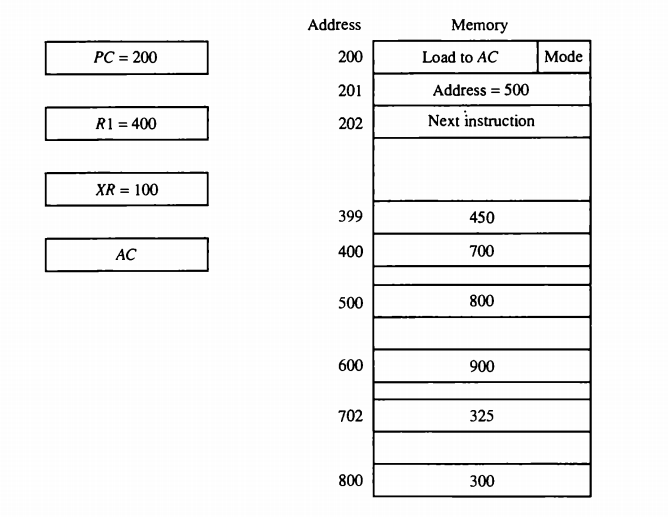
\includegraphics[scale=.7]{./AddressingModes.png}
	%\caption{}
\end{center}

\subsection{Direct Address Mode}
the effective address is the address part of the instruction 500 and the operand to be loaded into AC is 800.

\subsection{Immediate Mode}
the second part of the instruction is taken as the operand rather than an address, so 500 is loaded into AC.(The effective address in this case is 201)

\subsection{Indirect Mode}
the effective address is stored in memory at address 500.
Therefore, the effective address is 800 and the operand is 300.

\subsection{Relative Mode}
the effective address is 500+202=702
and the operand is 325

** Note that the value in PC after the fetch phase and during the execute phase is 202

\subsection{Index Mode}
the effective address is XR + 500 = 100 + 500 = 600
and the operand is 900


\subsection{Register Mode}
the operand is in R1 and 400 is loaded into AC

** There is no effective address in this case


\subsection{Register Indirect Mode}
the effective address 400, equal to the content of R1 and the operand loaded into AC is 700 .

\subsection{Autoincremented Mode}
is the same as register indirect mode except that R1 is incremented to 401 after the execution of the instruction.

\subsection{Autodecremented mode}
decrements R1 to 399 before of the execution of the instruction, and the operand loaded into AC is now 450

\end{document}